\documentclass[a4paper,UKenglish,cleveref, autoref, thm-restate]{lipics-v2021}
%This is a template for producing LIPIcs articles. 
%See lipics-v2021-authors-guidelines.pdf for further information.
%for A4 paper format use option "a4paper", for US-letter use option "letterpaper"
%for british hyphenation rules use option "UKenglish", for american hyphenation rules use option "USenglish"
%for section-numbered lemmas etc., use "numberwithinsect"
%for enabling cleveref support, use "cleveref"
%for enabling autoref support, use "autoref"
%for anonymousing the authors (e.g. for double-blind review), add "anonymous"
%for enabling thm-restate support, use "thm-restate"
%for enabling a two-column layout for the author/affilation part (only applicable for > 6 authors), use "authorcolumns"
%for producing a PDF according the PDF/A standard, add "pdfa"

%\pdfoutput=1 %uncomment to ensure pdflatex processing (mandatatory e.g. to submit to arXiv)
%\hideLIPIcs  %uncomment to remove references to LIPIcs series (logo, DOI, ...), e.g. when preparing a pre-final version to be uploaded to arXiv or another public repository

%\graphicspath{{./graphics/}}%helpful if your graphic files are in another directory

\bibliographystyle{plainurl}% the mandatory bibstyle

\title{What's in a Name? Linear Temporal Logic Literally Represents Time Lines} %TODO Please add

%\titlerunning{Dummy short title} %TODO optional, please use if title is longer than one line

\author{Runming Li\thanks{These authors contributed equally to this work}}{Carnegie Mellon University, USA}{runmingl@andrew.cmu.edu}{https://orcid.org/0000-0001-7600-9069}{}%TODO mandatory, please use full name; only 1 author per \author macro; first two parameters are mandatory, other parameters can be empty. Please provide at least the name of the affiliation and the country. The full address is optional. Use additional curly braces to indicate the correct name splitting when the last name consists of multiple name parts.

\author{Keerthana Gurushankar\footnotemark[1]}{Carnegie Mellon University, USA}{kgurusha@andrew.cmu.edu}{[orcid]}{}

\authorrunning{Li and Gurushankar} %TODO mandatory. First: Use abbreviated first/middle names. Second (only in severe cases): Use first author plus 'et al.'

\Copyright{Runming Li and Keerthana Gurushankar} %TODO mandatory, please use full first names. LIPIcs license is "CC-BY";  http://creativecommons.org/licenses/by/3.0/

\begin{CCSXML}
<ccs2012>
   <concept>
       <concept_id>10003752.10003766.10003770</concept_id>
       <concept_desc>Theory of computation~Automata over infinite objects</concept_desc>
       <concept_significance>500</concept_significance>
       </concept>
   <concept>
       <concept_id>10003752.10003766.10003776</concept_id>
       <concept_desc>Theory of computation~Regular languages</concept_desc>
       <concept_significance>300</concept_significance>
       </concept>
   <concept>
       <concept_id>10003752.10003790.10003793</concept_id>
       <concept_desc>Theory of computation~Modal and temporal logics</concept_desc>
       <concept_significance>500</concept_significance>
       </concept>
   <concept>
       <concept_id>10003752.10003790.10002990</concept_id>
       <concept_desc>Theory of computation~Logic and verification</concept_desc>
       <concept_significance>300</concept_significance>
       </concept>
 </ccs2012>
\end{CCSXML}

\ccsdesc[500]{Theory of computation~Automata over infinite objects}
\ccsdesc[300]{Theory of computation~Regular languages}
\ccsdesc[500]{Theory of computation~Modal and temporal logics}
\ccsdesc[300]{Theory of computation~Logic and verification}

\keywords{Linear Temporal Logic, \Buchi automata, $\omega$-regular expression, model checking, visualization} %TODO mandatory; please add comma-separated list of keywords

\category{} %optional, e.g. invited paper

\relatedversion{} %optional, e.g. full version hosted on arXiv, HAL, or other respository/website
%\relatedversiondetails[linktext={opt. text shown instead of the URL}, cite=DBLP:books/mk/GrayR93]{Classification (e.g. Full Version, Extended Version, Previous Version}{URL to related version} %linktext and cite are optional

%\supplement{}%optional, e.g. related research data, source code, ... hosted on a repository like zenodo, figshare, GitHub, ...
%\supplementdetails[linktext={opt. text shown instead of the URL}, cite=DBLP:books/mk/GrayR93, subcategory={Description, Subcategory}, swhid={Software Heritage Identifier}]{General Classification (e.g. Software, Dataset, Model, ...)}{URL to related version} %linktext, cite, and subcategory are optional

%\funding{(Optional) general funding statement \dots}%optional, to capture a funding statement, which applies to all authors. Please enter author specific funding statements as fifth argument of the \author macro.


\nolinenumbers %uncomment to disable line numbering



%Editor-only macros:: begin (do not touch as author)%%%%%%%%%%%%%%%%%%%%%%%%%%%%%%%%%%
\EventEditors{}
\EventNoEds{1}
\EventLongTitle{}
\EventShortTitle{}
\EventAcronym{}
\EventYear{}
\EventDate{}
\EventLocation{}
\EventLogo{}
\SeriesVolume{}
\ArticleNo{1}
%%%%%%%%%%%%%%%%%%%%%%%%%%%%%%%%%%%%%%%%%%%%%%%%%%%%%%
\usepackage{algorithm, algpseudocode, amsmath, amsfonts, scalerel}
\usepackage{hyperref}
\hypersetup{
    colorlinks=true,  
    urlcolor=blue,
    linkcolor=blue,
    citecolor=blue,
    pdfpagemode=FullScreen,
    }
\algrenewcommand\algorithmicrequire{\textbf{Input:}}
\algrenewcommand\algorithmicensure{\textbf{Output:}}
\crefname{algocf}{alg.}{algs.}
\Crefname{algocf}{Algorithm}{Algorithms}

\newcommand{\AP}{\mathcal{AP}}
\newcommand{\always}{\Box}
\newcommand{\eventually}{\Diamond}
\newcommand{\nextt}{\mathcal{X}}
\newcommand{\limplies}{\rightarrow}
\newcommand{\ltl}{\textit{LTL}}

\newcommand{\Buchi}{B\"{u}chi }
\newcommand{\stronguntil}{\hspace{0.1cm} \mathcal{U}  \hspace{0.1cm}}
\newcommand{\strongrelease}{\hspace{0.1cm} \mathcal{M} \hspace{0.1cm}}
\newcommand{\weakuntil}{\hspace{0.1cm} \mathcal{W} \hspace{0.1cm}}
\newcommand{\weakrelease}{\hspace{0.1cm} \mathcal{R} \hspace{0.1cm}}
\newcommand{\liff}{\leftrightarrow}
\DeclareMathOperator*{\bigplus}{\scalerel*{+}{\sum}}

% hyperref must go last
\usepackage{hyperref}
% but cleveref goes "laster" than hyperref
\usepackage[capitalise,noabbrev]{cleveref}
\providecommand\algorithmname{algorithm}
\crefname{algocf}{alg.}{algs.}
\Crefname{algocf}{Algorithm}{Algorithms}

\begin{document}

\maketitle


%TODO mandatory: add short abstract of the document
\begin{abstract}
    Linear Temporal Logic (\ltl) is widely used to specify requirements in safety-critical systems.
    However, like many formal verification techniques, it is known to be unintuitive and error-prone for human practitioners to specify and validate.
    In this paper, we provide a new timeline tool for visualizing \ltl-based specifications, which is effective at intuitively representing a wide range of formulas.
    Our tool generates timeline visualizations by translating \ltl\ formulae to intermediate representations as \Buchi automata and then $\omega$-regular expressions, and finally simplifying and visualizing the expressions.
    We provide an algorithm for this visualization, a theoretical soundness analysis, and an implementation.
\end{abstract}

\section{Introduction}

Formal methods, including Linear Temporal Logic (\ltl), are widely used in the specification and analysis of safety-critical systems, such as those found in the aerospace industry. These methods provide powerful tools for rigorously verifying the correctness of system designs, from early design-time model checking to on-board runtime verification. However, these methods can be difficult for humans to understand and use, leading to the possibility of errors and misunderstandings.

There has been recent work aimed at making the use of formal methods more intuitive for humans, such as NASA's FRET (Formal Requirements Engineering Tool) \cite{GPMS20} which uses structured natural language to bridge the gap between natural language and formal semantics. 

However, \ltl\ is a literally a language of timelines, so timeline visualizations have the potential to be a powerful tool for representing \ltl\ formulas in an intuitive manner. In this paper, we propose such a timeline visualization tool, using regular expressions, to effectively represent a wide range of \ltl-based formulas. 

\section{Setting the stage}

\subsection{Linear temporal logic (LTL)}

\begin{definition}[Linear Temporal Logic (LTL)]
    % cite Kristin's survey paper
    The syntax of an LTL formula over a set of atomic propositions $\AP$, where $p\in\AP$ is a propositional variable, is given by the following grammar:
    \begin{align*}
        \Phi ::= p \mid \neg \Phi \mid \Phi \land \Phi \mid \Phi \lor \Phi \mid \Phi \limplies \Phi \mid \always \Phi \mid \eventually \Phi \mid \nextt \Phi
    \end{align*}\label{ltl-defn}
\end{definition}
Intuitively, $\always \Phi$ says that formula $\Phi$ is true at every time step; $\eventually \Phi$ says that formula $\Phi$ is true either now or at sometime in the future time step; and $\nextt \Phi$ says formula $\Phi$ is true at the next time step immediately after the current one.
\begin{remark}
    The definition of \ltl\ can be extended to allow release and until as shown below, but they are definable using connectives in \ref{ltl-defn}, hence they are omitted in the definition. The tool we present in this paper, however, does support those operators.
    \begin{align*}
        \Phi ::= \cdots \mid \Phi \strongrelease \Phi \mid \Phi \stronguntil \Phi \mid \Phi \weakrelease \Phi \mid \Phi \weakuntil \Phi 
    \end{align*}
\end{remark}

\begin{definition}[Semantics of \ltl\ formula]
    The semantics of \ltl\ formula is defined via judgement $\pi, i \models \Phi$ where $\pi : \omega \rightarrow 2^{\AP}$ is the computation that stores the truthhood and falsehood of every atomic proposition at every time step, and $\omega$ is the set of natural numbers that denote the time step. The semantics follows exactly from \cite{Roz11}.
\end{definition}

\subsection{State-based \Buchi automata (BA)}
\begin{definition}[$\omega$-word]
    An $\omega$-word or infinite run of $\Sigma$, is an infinite string $s = (s_0, s_1, s_2, \dots)$ where each $s_i\in \Sigma$
\end{definition}
\begin{definition}[\Buchi automaton]
    A \Buchi automaton is a $5$-tuple, $G = (Q, \Sigma, \delta, s, F)$ consisting of
    \begin{enumerate}
        \item a finite set of states $Q$
        \item a finite alphabet of input symbols called the alphabet $\Sigma$
        \item a partial function $\delta : Q\times \Sigma \to Q$, called the transition function
        \item an initial or start stae called $s\in Q$
        \item a set of accept states $F \subseteq Q$
    \end{enumerate}
    $G$ accepts an infinite run iff at least one of its infinitely visited states is in $F$
\end{definition}
\subsection{$\omega$-regular expression}
\begin{definition}[Regular expression]
    For word $a \in \Sigma$, regular expression is defined by the following grammar:
    \begin{align*}
        A ::= \emptyset \mid \epsilon \mid a \mid AA \mid A + A \mid A^*
    \end{align*}
\end{definition}
\begin{definition}[Semantics of regular expression]
    Let $L(A)$ denote the language accepted by regular expression $A$. Then $L(A)$ is inductively defined as
    \begin{align*}
        L(\emptyset) & = \emptyset \\
        L(\epsilon) & = \{\epsilon\} \\
        L(a) & = \{a\} \\
        L(A_1A_2) & = \{s_1s_2 \mid s_1 \in L(A_1) \text{ and } s_2 \in L(A_2)\} \\
        L(A_1 + A_2) & = L(A_1) \cup L(A_2) \\
        L^{(0)}(A) & = \{\epsilon\} \\
        L^{(i + 1)}(A) & = \{s_1s_2 \mid s_1 \in L(A) \text{ and } s_2 \in L^{(i)}(A)\} \\\
        L(A^*) & = \bigcup_{i \ge 0} L^{(i)}(A)
    \end{align*}
\end{definition}

\begin{remark}
    For the purpose of our tool, $\Sigma$ is the set of propositional logic formula defined as
    \[
    \Psi ::= p \mid \neg \Psi \mid \Psi \land \Psi \mid \Psi \lor \Psi \mid \Psi \limplies \Psi
    \]
\end{remark}

\begin{definition}[$\omega$-regular expression]
    Regular expression concerns only finite-length strings. However, since \ltl\ formulas reason about events that happen over an infinite-length timeline, we need to model it using infinite regular expressions (i.e. $\omega$-regular expression). $\omega$-regular expression is defined by the following grammar:
    \begin{align*}
        B ::= A^{\omega} \mid AB \mid B + B
    \end{align*}
\end{definition}
\begin{definition}[Semantics of $\omega$-regular expression]\label{def:omega-semantics}
    Let $\Sigma^{\omega}$ denote the set of infinite-length string over fixed alphabet $\Sigma$. Let $L_{\omega}(B)$ denote the $\omega$-language accepted by $\omega$-regular expression $B$. Then $L_{\omega}(B)$ is inductively defined as
    \begin{align*}
        L_{\omega}(A^{\omega}) & = \{s_1s_2s_3\cdots \mid s_i \in L(A) \text{ and } i \ge 1\} \\
        L_{\omega}(AB) & = \{s_1s_2 \mid s_1 \in L(A) \text{ and } s_2 \in L_{\omega}(B)\} \\
        L_{\omega}(B_1 + B_2) &= L_{\omega}(B_1) \cup L_{\omega}(B_2) 
    \end{align*}
\end{definition}

\subsection{Timeline}
We present timelines as graphic visualizations. It contains the following features:
\begin{itemize}
    \item Every timeline starts with a node named ``start''.
    \item Every node represents one time step, and each node has a propositional logic formula $\Psi$, which specifies the behavior of atomic propositions at that time step. The formula $\Psi$ must be true at that time step. If $\Psi = 1$, that means all atomic propositions can behave arbitrarily.
    \item A node with label ``$\cdots$'' means to repeat the node prior to it and after it finitely many times.
    \item The grey box means repeat infinitely. Once we reach the end of a timeline in the grey box, we must reenter the same grey box from any of its starting point.
\end{itemize}

\begin{example}
    In figure \ref{fig:ex2}, one can reason about two timelines: the upper timeline starts with $p$ at the first time step, followed by entering the grey box with one step of $!p$ and one step of $p$. Then at the end of the grey box, we reenter the box, with the next time step being $!p$, and so on. The lower timeline starts with one step of $!p$ and one step of $p$ outside the grey box, and then enter the infinite run of $!p$ and $p$ repeating. 
    \begin{figure}[h!]
        \centering
        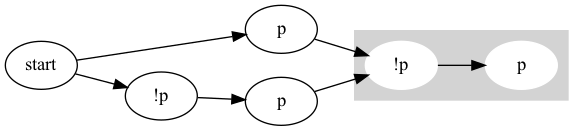
\includegraphics[scale=0.4]{examples/ex2/ex2.gv.png}
        \caption{Example timeline for specification ``$p$ oscillates every time step''}
        \label{fig:ex2}
    \end{figure}
\end{example}

\section{Algorithm}
On a high level, our algorithm of converting \ltl\ formula into timeline visualization works as follows:
\begin{enumerate}
    \item Convert \ltl\ formula to its corresponding \Buchi automata \ref{ltl2aut}
    \item Derive the $\omega$-regular expression corresponding to the \Buchi automata \ref{aut2regex}
    \item Simplify the derived $\omega$-regular expression \ref{regex-simplify}
    \item Visualize the $\omega$-regular expression according to its structure \ref{regex2timeline}
\end{enumerate}
\begin{figure}[h!]
    \centering
    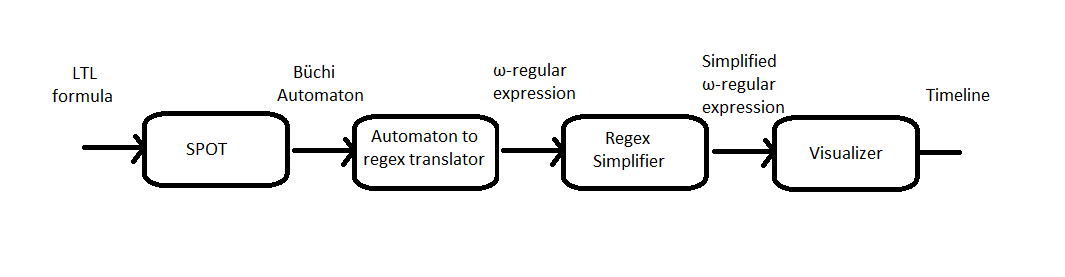
\includegraphics[scale=0.5]{img/algo-flowchart.png}
    \caption{Algorithm outline}
    \label{fig:algo}
\end{figure}
\subsection{LTL to BA} \label{ltl2aut}
The translation from LTL formulas to \Buchi automata is provided by SPOT\cite{Dur22}\footnote{For our tool, we use SPOT version 2.11.}.

\subsection{BA to $\omega$-regex} \label{aut2regex}

We translate \Buchi automata to $\omega$-regular expressions by first finding the regular expressions for paths from the start state to some final state (say $r_{sf}$), and for those for paths for looping from the final state back to itself (say $r_{ff}$), and finally combining those to form the $\omega$-expression for valid runs ($\bigplus_{f\in F} r_{sf}r_{ff}^\omega$). The regular expressions for finite paths are in turn found by iteratively deleting interior nodes in digraph of the automaton. 

The algorithm is outlined below (see Algorithms 1 - 4). %\cref{alg:ba2wregex}

\begin{algorithm}[h!]
    \caption{reduce\_dfa}
    \begin{algorithmic}
        \Require ($G, v$), a DFA with state $v$ that is not initial or final
        \Ensure Deletes state $v$ from $G$ while ensuring the same language is recognized
        \For{ every $u\xrightarrow{r_{in}} v, v \xrightarrow{r_{out}} w$ }
            \If {$v$ has a self-edge  $v\xrightarrow{r_{loop}}v$}
                \State replace edges $u\xrightarrow{r_{in}} v, v \xrightarrow{r_{out}} w$ with $u \xrightarrow{r_{in} r_{loop}* r_{out}} w$
            \Else
                \State replace edges $u\xrightarrow{r_{in}} v, v \xrightarrow{r_{out}} w$ with $u \xrightarrow{r_{in}  r_{out}} w$
            \EndIf
        \EndFor
        %\State \Return the reduced graph $G$
    \end{algorithmic}
\end{algorithm}
\begin{algorithm}[h!]
    \caption{dfa2regex}
    \begin{algorithmic}
        \Require ($G, s, f$), a DFA with initial state $s$ and final state $f$
        \Ensure The regular expression corresponding to all paths from $s$ to $f$
        % WHile there exists any edge except r_sf
        \While{ there exists an interior vertex $v$ }
            \State reduce\_dfa($G, v$)
            \State combine multiedges, i.e. $r1 : u \to w, r2 : u \to w$  to $r1 | r2 : u \to w$
        \EndWhile
        \State \Return $(r_{ss}| r_{sf} r_{ff}^* r_{fs})^* r_{sf} r_{ff}$
        % if called by first visit, this is r_{ss}* r_{sf}
        % if called by ba2wregex, s=f, this is r_{ff}
        % consider modularizing fns differently
        % \State \Return regexp labelling the edge $s\to f$
    \end{algorithmic}
\end{algorithm}
\begin{algorithm}[h!]
    \caption{dfa2regex\_firstvisit}
    \begin{algorithmic}
        \Require ($G, s, f$), a DFA with initial state $s$ and final state $f$
        \Ensure The regular expression of all paths from $s$ reaching $f$ for the first time
        \State delete all out edges from $f$ in $G$
        \State \Return dfa2regex($G, s, f$)
    \end{algorithmic}
\end{algorithm}
\begin{algorithm}[h!]
    \label{alg:ba2wregex}
    \caption{ba2wregex}
    \begin{algorithmic}
        \Require $G$, a \Buchi automaton
        \Ensure The $\omega$-regular expression recognized by $G$
        \State \Return $\bigcup_{f \in F}\left({\verb|dfa2regex_firstvisit|}(G, s, f){\verb|^dfa2regex|}(G, f, f) \right) $
    \end{algorithmic}
\end{algorithm}

\subsection{$\omega$-regex simplification} \label{regex-simplify}
The $\omega$-regular expression generated in \ref{aut2regex} may not be the ``simplest'' for the purpose of visualizing the timeline. We have observed multiple patterns in the resulting $\omega$-regular expression that could be simplified. For example, an $\omega$-regular expression in the form of $r^*r^{\omega}$ represents the same timeline as $r^{\omega}$, but the latter is more intuitive. For this purpose, we devised some simplification rules in our tool, based on our observation of common patterns in the generated $\omega$-regular expression.
\paragraph*{Rule-based simplification}
Here we show a demonstrating subset of simplification rules we encoded.
\begin{alignat*}{2}
        & r_1 + r_1r_2^* && \Longrightarrow r_1r_2^* \\
        & r + r && \Longrightarrow r \\
        & r_1 + r_2^*r_1 && \Longrightarrow r_2^*r_1 \\
        & (r^*)^{\omega} && \Longrightarrow r^{\omega} \\
        & (r_1r_2^*)r_2^{\omega} && \Longrightarrow r_1r_2^{\omega} \\
        & (r_1r_2)r_2^{\omega} && \Longrightarrow r_1r_2^{\omega} \\
        & r^*r^{\omega} && \Longrightarrow r^{\omega} \\
        & rr^{\omega} && \Longrightarrow r^{\omega}
\end{alignat*}
\paragraph*{Result of simplification}
Those simplification rules lead to more intuitive representation of timelines. Here we demonstrate their effects using an example. 
\begin{example}
    The formula $\Phi = \always (a \limplies \eventually (\neg a))$ generates un-simplified $\omega$-regular expression $((!a) | ((aa^*(!a)))((!a) | ((aa^*(!a)))^{\omega}$, and simplified version $((!a) | ((aa^*(!a)))^{\omega}$, which corresponds to the two timelines in figure \ref{fig:unsimplified} and \ref{fig:simplified}.
    \begin{figure}[h!]
        \centering
        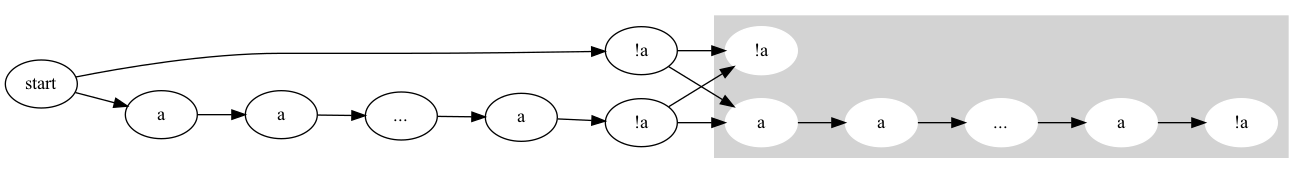
\includegraphics[scale=0.3]{examples/ex9/ex9-unsimplified.gv.png}
        \caption{Timeline for un-simplified $\omega$-regular expression $((!a) | ((aa^*(!a)))((!a) | ((aa^*(!a)))^{\omega}$}
        \label{fig:unsimplified}
    \end{figure}
    \begin{figure}[h!]
        \centering
        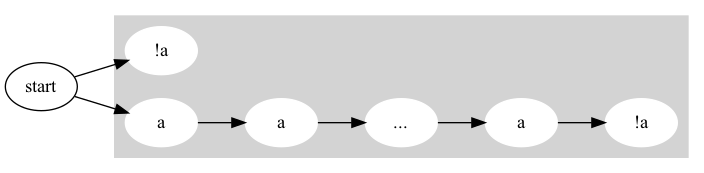
\includegraphics[scale=0.3]{examples/ex9/ex9.gv.png}
        \caption{Timeline for simplified $\omega$-regular expression $((!a) | ((aa^*(!a)))^{\omega}$}
        \label{fig:simplified}
    \end{figure}
\end{example}

\begin{remark}
    Both simplified and un-simplified $\omega$-regular expression would generate correct timeline representations. Correct as they faithfully represent the set of satisfying traces of the original \ltl\ formula $\Phi$. Nonetheless, we, as human user, oftentimes find the simplified version more intuitive to reason about.
\end{remark}

\subsection{$\omega$-regex to timeline} \label{regex2timeline}
Our tool uses Graphviz\cite{Ellson2001GraphvizO} to achieve the timeline visualization step. By construction of our algorithm, every $\omega$-regular expression is in the form of 
\[
    A_1A_2^{\omega} + A_3A_4^{\omega} + \cdots + A_{2n-1}A_{2n}^{\omega}
\]
where $A_i$ are regular expressions, and $A_{2i-1}$ could be $\epsilon$. On a high level, for each of regular expression $A_i$, we visualize it as a set of accepted input. We view each union operator as parallel timelines, and each $A_{2i-1}$ is concatenated with $A_{2i}$ repeated infinitely many times, as represented in the grey box. Figure \ref{fig:timeline} presents a generic timeline resulting from this form of construction.
\begin{figure}[h!]
    \centering
    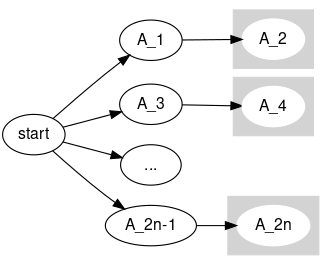
\includegraphics[scale=0.5]{img/timeline.png}
    \caption{Generic timeline construction from $A_1A_2^{\omega} + A_3A_4^{\omega} + \cdots + A_{2n-1}A_{2n}^{\omega}$}
    \label{fig:timeline}
\end{figure}


\section{Theoretical Analyses}
\subsection{Correctness of Regex Translation}
\begin{lemma}
    % reduce_dfa does its input to output behaviour
    For any DFA $G$ and any state $v$ in $G$ that is neither a start state or a final state, \textbf{reduce\_dfa}$(G, v)$ preserves the regular language accepted by $G$
\end{lemma}
\begin{proof}
    Let $G'$ be the graph of $G$ post reduction by the application of \textbf{reduce\_dfa}$(G, v)$. We show that the trace of every path accepted by $G$ is also accepted by $G'$. Suppose a path accepted by $G$ does not pass through $v$, clearly this is true. Else, suppose it passes through $v$, since $v$ is an interior node, $v$ cannot be the first or last in the path. Thus, for every pass through $v$, let $u\neq v$ be the last node passed before entering $v$, and likewise $w$ be the first node after exiting $v$. We show that the regular language of sub-traces from $u$ to $w$ in $G$ (shown in \cref{fig:uvw-dfa}) is identical to that in $G'$. 
    \begin{figure}[h!]
        \centering
        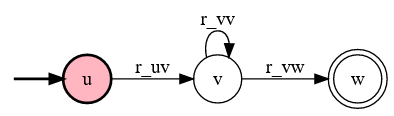
\includegraphics[scale=0.5]{img/uvw-dfa.png}
        \caption{$u$ to $w$ path in $G$}
        \label{fig:uvw-dfa}
    \end{figure}
    Suppose there is no loop at $v$, the path from $u$ to $w$ must simply be $u\xrightarrow{r_{uv}}v\xrightarrow{r_{vw}}w$, with the trace $r=r_{uv}r_{vw}$. If there is a loop edge $r_{vv}$, this edge can be travelled any number of times before exiting $v$, thus the regular expression is $r=r_{uv}r_{vv}^*r_{vw}$. This edge $u\xrightarrow{r}w$ is added in $G'$. Thus, for every path accepted by $G$, for every subpath entering and exiting $v$ from some $u$ to $w$, there exists a corresponding subpath from $u$ to $w$ in $G'$, and thus a corresponding path accepted by $G'$. 
\end{proof}

\begin{lemma}
    For any DFA $G$ with start state $s$ and (exactly one) final state $f$, \textbf{dfa2regex}$(G, s, f)$ outputs the regular expression of all paths from $s$ to $f$ (i.e., the language accepted by $G$)
\end{lemma}
\begin{proof}
    The while loop clearly terminates since the number of interior nodes is strictly decreasing, and upon termination, $G$ is a DFA containing only the nodes $s$ and $f$. Now, every non-terminal visit from $s$ to $f$ and back to $s$, can be replaced by an edge $s\xrightarrow{r_{sf}r_{ff}^* r_{fs}} s$, instead of the edge $f\to s$. This DFA yields the regular language $(r_{ss}|r_{sf}r_{ff}^* r_{fs})^* r_{sf} r_{ff}$, as outputted by the algorithm. 
\end{proof}

\begin{lemma}
    For any DFA $G$ with start state $s$ and (exactly one) final state $f$, \\\textbf{dfa2regex\_firstvisit}$(G, s, f)$ outputs the regular expression of all paths from $s$ to $f$, visiting $f$ for the first time.
\end{lemma}
\begin{proof}
    Let $G'$ be $G$ with all out-edge (including loops) from $f$ deleted. We claim that $L(G')$ is equal to the language $L'$ of all paths from $s$ reaching $f$ for the first time. 

    First we show $L(G') \subseteq L'$, i.e., every path accepted by $G'$ starts in $s$ and ends by reaching $f$ for the first time. Since $s$ and $f$ are the initial and final states of $G'$ respectively, clearly every path accepted by $G$ must start in $s$ and end in $f$. Further, as $f$ has no out-edges in $G$, any accepted path must end immediately once it reaches $f$. Thus it must end once it reaches $f$ for the first time. 

    Also, we show $L' \subseteq L(G')$, i.e., every path starting in $s$ and ending by $f$ reaching $f$ for the first time is accepted by $G'$. If a path contains an out-edge of $f$, it cannot be in $L'$ as the trace continues beyond the first time step at $f$. Thus, every trace in $L'$ only uses edges in $G'$, and is thus accepted by $G$ iff it is accepted by $G'$. 
\end{proof}

\begin{theorem}
    For any \Buchi automaton $G$ with start state $s$ and final states $F$, \textbf{ba2wregex}$(G)$ outputs the $\omega$-regular language accepted by $G$
\end{theorem}
\begin{proof}
    We show that $L = \bigcup_{f\in F} \textbf{dfa2regex}(G, s, f)$ \verb|^| $\left(\textbf{dfa2regex\_firstvisit}(G, f, f)\right)^\omega$ and the $\omega$-language accepted by $G$, $L_\omega(G)$ are identical. 
    
    First, $L\subseteq L_\omega(G)$ since for every infinite run in $L$, clearly by definition of $L$, there is some $f\in F$ such that passes through $f$ infinitely often. The converse is true as well: for every infinite run $q_0, q_1, \dots$ accepted by $G$, then $q_0 = s$ and by definition of the accepting language, there is some accepting state $f$, passed through infinitely often, thus the run is in $\textbf{dfa2regex}(G, s, f)$ \verb|^| $\left(\textbf{dfa2regex\_firstvisit}(G, f, f)\right)^\omega$
\end{proof}
\subsection{Correctness of Rewrite Rules}
\begin{lemma}
    For all regular expressions $r_1, r_2, r$, each of the following rewrite rules preserve the regular or $\omega$-regular language represented by the expressions:
    \begin{alignat}{2}
        & r_1 + r_1r_2^* && \Longrightarrow r_1r_2^* \\
        & r + r && \Longrightarrow r \\
        & r_1 + r_2^*r_1 && \Longrightarrow r_2^*r_1 \\
        & (r^*)^{\omega} && \Longrightarrow r^{\omega} \\
        & (r_1r_2^*)r_2^{\omega} && \Longrightarrow r_1r_2^{\omega} \\
        & (r_1r_2)r_2^{\omega} && \Longrightarrow r_1r_2^{\omega} \\
        & r^*r^{\omega} && \Longrightarrow r^{\omega} \\
        & rr^{\omega} && \Longrightarrow r^{\omega}
    \end{alignat}
\end{lemma}

The soundness of each of these translations can be proven by reasoning about the  semantics detailed in \cref{def:omega-semantics}. A full proof is not provided at this time. 


%\begin{theorem}
%    For any LTL formula $\phi$, 
%\end{theorem}

\section{Tool showcase}
To demonstrate the result of our tool, we present two examples, one from a real-world model checking example in \cite{ZR14} and one from a randomly generated \ltl\ formula.

\begin{example}
    \cite{ZR14} presents a model verification specification says ``[i]f a TSAFE command is sent to an aircraft, controller/AutoResolver should then hand off the control of this aircraft'' which corresponds to \ltl\ formula 
    \[
    \always (\texttt{tsafe.TSAFE\_command1} \land \texttt{controller.CTR\_control\_1} \limplies \nextt (\neg \texttt{controller.CTR\_control\_1}))
    \]
    For simplicity, we swap the concrete atomic proposition to $a, b, c$ and get
    \[
    \always (a \land b \limplies \nextt (\neg b))
    \]
    For this \ltl\ formula, our tool generates the timeline representation in figure \ref{fig:ex14}.
    \begin{figure}[h!]
        \centering
        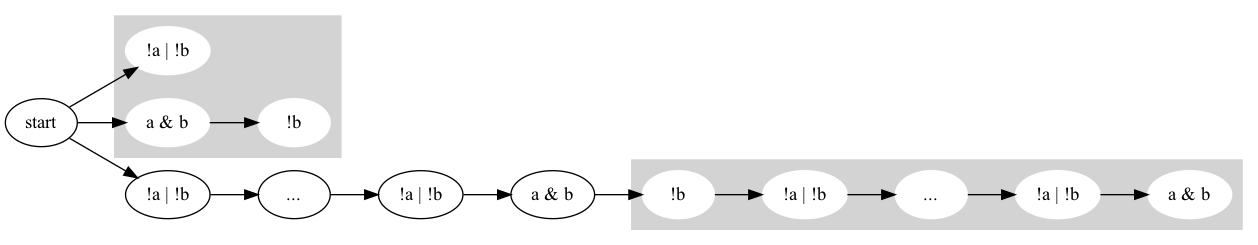
\includegraphics[scale=0.3]{examples/ex14/ex14.gv.png}
        \caption{Timeline for $\always (a \land b \limplies \nextt (\neg b))$}
        \label{fig:ex14}
    \end{figure}
\end{example}

\begin{example}
    Spot \cite{SPOT-online} presents command-line tool for random \ltl\ formula generator \texttt{randltl}\cite{duret.13.atva}. The following \ltl\ formula is generated from this tool. 
    \[
    p_2 \land (\eventually (\always p_0 \strongrelease  1) \weakrelease \nextt(\always p_1 \land ((p_0 \liff p_2) \stronguntil \eventually p_0)))
    \]
    This formula is reasonably complicated, and hard for human to reason about directly. For this \ltl\ formula, our tool generates the timeline representation in figure \ref{fig:ex13}.
    \begin{figure}[h!]
        \centering
        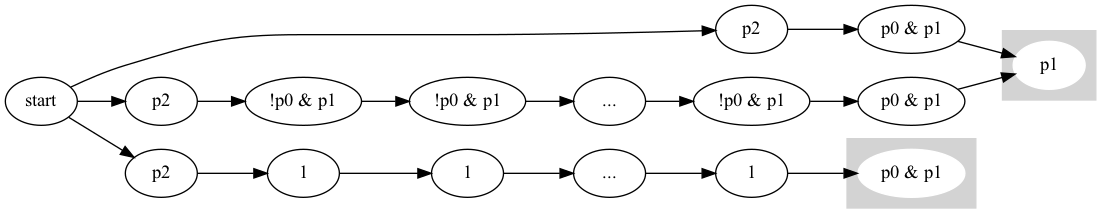
\includegraphics[scale=0.3]{examples/ex13/ex13.gv.png}
        \caption{Timeline for $p_2 \land (\eventually (\always p_0 \strongrelease  1) \weakrelease \nextt(\always p_1 \land ((p_0 \liff p_2) \stronguntil \eventually p_0)))$}
        \label{fig:ex13}
    \end{figure}
\end{example}
\begin{remark}
    These two examples show that our tool can generate reasonably clear diagrams for both real-world formula and randomly generated formula.
\end{remark}

\section{Artifact availability}
The tool we present in this paper is available at 
\[
\text{\url{https://github.com/EULIR/ltl-explainability}}
\]
which comes with two command-line tools, \texttt{ltl2regex} and \texttt{ltl2timeline}. The specific usage of the tool can be found  \href{https://github.com/EULIR/ltl-explainability#usage}{here}.


\section{Future work}
Based on our results, we raise the following questions as future works:
\begin{itemize}
    \item Can there be more simplifications methods as described in \ref{regex-simplify}? The answer is definitely positive. On one hand, more rule-based simplifications can be discovered by finding more patterns in the generated $\omega$-regular expressions. On the other hand, other simplification are possible: for example, if the generated $\omega$-regular expression is $r_1 + r_2$ where $r_1, r_2$ are not syntactically equivalent (or equivalent up to algebraic rules) $\omega$-regular expressions, but they accepts the same set of infinite-length strings, then we can simplify this down to just $r_1$. This reduce the problem to equivalence test on $\omega$-regular expressions, which is decidable. In the similar vein, many more simplifications can be used, but the question is how efficient are they? In the end, one have to balance trade-off between the efficiency of the tool and the simplicity of the result.
    %\item Our tool is effective at translating a wide range of LTL formulas. Even with LTL formulae with complex nesting structure are represented by relatively readable timeline visualizations. 
    \item Can we define timeline more formally so that one can do this process reversely (i.e. a tool that converts timeline representation to its corresponding \ltl\ formula)? That would be a very useful tool in practice. However, a direct reverse of the algorithm we presented in this paper may not be viable.
\end{itemize}

\section{Acknowledgement}
We sincerely appreciate the guidance of Professors Kristin Yvonne Rozier and Marijn Heule throughout our project.

\bibliography{Related Work}
% \cite{*} %?
\end{document}








%%%%%%%%%%%%%%%%%%%%%%%%%%%%%%%%%%%%%%%%%%%%%%%%%%%%%%%%%%%%%%%%%%%%%%
\section{Typesetting instructions -- Summary}
\label{sec:typesetting-summary}

LIPIcs is a series of open access high-quality conference proceedings across all fields in informatics established in cooperation with Schloss Dagstuhl. 
In order to do justice to the high scientific quality of the conferences that publish their proceedings in the LIPIcs series, which is ensured by the thorough review process of the respective events, we believe that LIPIcs proceedings must have an attractive and consistent layout matching the standard of the series.
Moreover, the quality of the metadata, the typesetting and the layout must also meet the requirements of other external parties such as indexing service, DOI registry, funding agencies, among others. The guidelines contained in this document serve as the baseline for the authors, editors, and the publisher to create documents that meet as many different requirements as possible. 

Please comply with the following instructions when preparing your article for a LIPIcs proceedings volume. 
\paragraph*{Minimum requirements}

\begin{itemize}
\item Use pdflatex and an up-to-date \LaTeX{} system.
\item Use further \LaTeX{} packages and custom made macros carefully and only if required.
\item Use the provided sectioning macros: \verb+\section+, \verb+\subsection+, \verb+\subsubsection+, \linebreak \verb+\paragraph+, \verb+\paragraph*+, and \verb+\subparagraph*+.
\item Provide suitable graphics of at least 300dpi (preferably in PDF format).
\item Use BibTeX and keep the standard style (\verb+plainurl+) for the bibliography.
\item Please try to keep the warnings log as small as possible. Avoid overfull \verb+\hboxes+ and any kind of warnings/errors with the referenced BibTeX entries.
\item Use a spellchecker to correct typos.
\end{itemize}

\paragraph*{Mandatory metadata macros}
Please set the values of the metadata macros carefully since the information parsed from these macros will be passed to publication servers, catalogues and search engines.
Avoid placing macros inside the metadata macros. The following metadata macros/environments are mandatory:
\begin{itemize}
\item \verb+\title+ and, in case of long titles, \verb+\titlerunning+.
\item \verb+\author+, one for each author, even if two or more authors have the same affiliation.
\item \verb+\authorrunning+ and \verb+\Copyright+ (concatenated author names)\\
The \verb+\author+ macros and the \verb+\Copyright+ macro should contain full author names (especially with regard to the first name), while \verb+\authorrunning+ should contain abbreviated first names.
\item \verb+\ccsdesc+ (ACM classification, see \url{https://www.acm.org/publications/class-2012}).
\item \verb+\keywords+ (a comma-separated list of keywords).
\item \verb+\relatedversion+ (if there is a related version, typically the ``full version''); please make sure to provide a persistent URL, e.\,g., at arXiv.
\item \verb+\begin{abstract}...\end{abstract}+ .
\end{itemize}

\paragraph*{Please do not \ldots} %Do not override the \texttt{\seriesstyle}-defaults}
Generally speaking, please do not override the \texttt{lipics-v2021}-style defaults. To be more specific, a short checklist also used by Dagstuhl Publishing during the final typesetting is given below.
In case of \textbf{non-compliance} with these rules Dagstuhl Publishing will remove the corresponding parts of \LaTeX{} code and \textbf{replace it with the \texttt{lipics-v2021} defaults}. In serious cases, we may reject the LaTeX-source and expect the corresponding author to revise the relevant parts.
\begin{itemize}
\item Do not use a different main font. (For example, the \texttt{times} package is forbidden.)
\item Do not alter the spacing of the \texttt{lipics-v2021.cls} style file.
\item Do not use \verb+enumitem+ and \verb+paralist+. (The \texttt{enumerate} package is preloaded, so you can use
 \verb+\begin{enumerate}[(a)]+ or the like.)
\item Do not use ``self-made'' sectioning commands (e.\,g., \verb+\noindent{\bf My+ \verb+Paragraph}+).
\item Do not hide large text blocks using comments or \verb+\iffalse+ $\ldots$ \verb+\fi+ constructions. 
\item Do not use conditional structures to include/exclude content. Instead, please provide only the content that should be published -- in one file -- and nothing else.
\item Do not wrap figures and tables with text. In particular, the package \texttt{wrapfig} is not supported.
\item Do not change the bibliography style. In particular, do not use author-year citations. (The
\texttt{natbib} package is not supported.)
\end{itemize}

\enlargethispage{\baselineskip}

This is only a summary containing the most relevant details. Please read the complete document ``LIPIcs: Instructions for Authors and the \texttt{lipics-v2021} Class'' for all details and don't hesitate to contact Dagstuhl Publishing (\url{mailto:publishing@dagstuhl.de}) in case of questions or comments:
\href{http://drops.dagstuhl.de/styles/lipics-v2021/lipics-v2021-authors/lipics-v2021-authors-guidelines.pdf}{\texttt{http://drops.dagstuhl.de/styles/lipics-v2021/\newline lipics-v2021-authors/lipics-v2021-authors-guidelines.pdf}}

\section{Lorem ipsum dolor sit amet}

Lorem ipsum dolor sit amet, consectetur adipiscing elit \cite{DBLP:journals/cacm/Knuth74}. Praesent convallis orci arcu, eu mollis dolor. Aliquam eleifend suscipit lacinia. Maecenas quam mi, porta ut lacinia sed, convallis ac dui. Lorem ipsum dolor sit amet, consectetur adipiscing elit. Suspendisse potenti. Donec eget odio et magna ullamcorper vehicula ut vitae libero. Maecenas lectus nulla, auctor nec varius ac, ultricies et turpis. Pellentesque id ante erat. In hac habitasse platea dictumst. Curabitur a scelerisque odio. Pellentesque elit risus, posuere quis elementum at, pellentesque ut diam. Quisque aliquam libero id mi imperdiet quis convallis turpis eleifend. 

\begin{lemma}[Lorem ipsum]
\label{lemma:lorem}
Vestibulum sodales dolor et dui cursus iaculis. Nullam ullamcorper purus vel turpis lobortis eu tempus lorem semper. Proin facilisis gravida rutrum. Etiam sed sollicitudin lorem. Proin pellentesque risus at elit hendrerit pharetra. Integer at turpis varius libero rhoncus fermentum vitae vitae metus.
\end{lemma}

\begin{proof}
Cras purus lorem, pulvinar et fermentum sagittis, suscipit quis magna.


\proofsubparagraph*{Just some paragraph within the proof.}
Nam liber tempor cum soluta nobis eleifend option congue nihil imperdiet doming id quod mazim placerat facer possim assum. Lorem ipsum dolor sit amet, consectetuer adipiscing elit, sed diam nonummy nibh euismod tincidunt ut laoreet dolore magna aliquam erat volutpat.
\begin{claim}
content...
\end{claim}
\begin{claimproof}
content...
    \begin{enumerate}
        \item abc abc abc \claimqedhere{}
    \end{enumerate}
\end{claimproof}

\end{proof}

\begin{corollary}[Curabitur pulvinar, \cite{DBLP:books/mk/GrayR93}]
\label{lemma:curabitur}
Nam liber tempor cum soluta nobis eleifend option congue nihil imperdiet doming id quod mazim placerat facer possim assum. Lorem ipsum dolor sit amet, consectetuer adipiscing elit, sed diam nonummy nibh euismod tincidunt ut laoreet dolore magna aliquam erat volutpat.
\end{corollary}

\begin{proposition}\label{prop1}
This is a proposition
\end{proposition}

\autoref{prop1} and \cref{prop1} \ldots

\subsection{Curabitur dictum felis id sapien}

Curabitur dictum \cref{lemma:curabitur} felis id sapien \autoref{lemma:curabitur} mollis ut venenatis tortor feugiat. Curabitur sed velit diam. Integer aliquam, nunc ac egestas lacinia, nibh est vehicula nibh, ac auctor velit tellus non arcu. Vestibulum lacinia ipsum vitae nisi ultrices eget gravida turpis laoreet. Duis rutrum dapibus ornare. Nulla vehicula vulputate iaculis. Proin a consequat neque. Donec ut rutrum urna. Morbi scelerisque turpis sed elit sagittis eu scelerisque quam condimentum. Pellentesque habitant morbi tristique senectus et netus et malesuada fames ac turpis egestas. Aenean nec faucibus leo. Cras ut nisl odio, non tincidunt lorem. Integer purus ligula, venenatis et convallis lacinia, scelerisque at erat. Fusce risus libero, convallis at fermentum in, dignissim sed sem. Ut dapibus orci vitae nisl viverra nec adipiscing tortor condimentum \cite{DBLP:journals/cacm/Dijkstra68a}. Donec non suscipit lorem. Nam sit amet enim vitae nisl accumsan pretium. 

\begin{lstlisting}[caption={Useless code.},label=list:8-6,captionpos=t,float,abovecaptionskip=-\medskipamount]
for i:=maxint to 0 do 
begin 
    j:=square(root(i));
end;
\end{lstlisting}

\subsection{Proin ac fermentum augue}

Proin ac fermentum augue. Nullam bibendum enim sollicitudin tellus egestas lacinia euismod orci mollis. Nulla facilisi. Vivamus volutpat venenatis sapien, vitae feugiat arcu fringilla ac. Mauris sapien tortor, sagittis eget auctor at, vulputate pharetra magna. Sed congue, dui nec vulputate convallis, sem nunc adipiscing dui, vel venenatis mauris sem in dui. Praesent a pretium quam. Mauris non mauris sit amet eros rutrum aliquam id ut sapien. Nulla aliquet fringilla sagittis. Pellentesque eu metus posuere nunc tincidunt dignissim in tempor dolor. Nulla cursus aliquet enim. Cras sapien risus, accumsan eu cursus ut, commodo vel velit. Praesent aliquet consectetur ligula, vitae iaculis ligula interdum vel. Integer faucibus faucibus felis. 

\begin{itemize}
\item Ut vitae diam augue. 
\item Integer lacus ante, pellentesque sed sollicitudin et, pulvinar adipiscing sem. 
\item Maecenas facilisis, leo quis tincidunt egestas, magna ipsum condimentum orci, vitae facilisis nibh turpis et elit. 
\end{itemize}

\begin{remark}
content...
\end{remark}

\section{Pellentesque quis tortor}

Nec urna malesuada sollicitudin. Nulla facilisi. Vivamus aliquam tempus ligula eget ornare. Praesent eget magna ut turpis mattis cursus. Aliquam vel condimentum orci. Nunc congue, libero in gravida convallis \cite{DBLP:conf/focs/HopcroftPV75}, orci nibh sodales quam, id egestas felis mi nec nisi. Suspendisse tincidunt, est ac vestibulum posuere, justo odio bibendum urna, rutrum bibendum dolor sem nec tellus. 

\begin{lemma} [Quisque blandit tempus nunc]
Sed interdum nisl pretium non. Mauris sodales consequat risus vel consectetur. Aliquam erat volutpat. Nunc sed sapien ligula. Proin faucibus sapien luctus nisl feugiat convallis faucibus elit cursus. Nunc vestibulum nunc ac massa pretium pharetra. Nulla facilisis turpis id augue venenatis blandit. Cum sociis natoque penatibus et magnis dis parturient montes, nascetur ridiculus mus.
\end{lemma}

Fusce eu leo nisi. Cras eget orci neque, eleifend dapibus felis. Duis et leo dui. Nam vulputate, velit et laoreet porttitor, quam arcu facilisis dui, sed malesuada risus massa sit amet neque.

\section{Morbi eros magna}

Morbi eros magna, vestibulum non posuere non, porta eu quam. Maecenas vitae orci risus, eget imperdiet mauris. Donec massa mauris, pellentesque vel lobortis eu, molestie ac turpis. Sed condimentum convallis dolor, a dignissim est ultrices eu. Donec consectetur volutpat eros, et ornare dui ultricies id. Vivamus eu augue eget dolor euismod ultrices et sit amet nisi. Vivamus malesuada leo ac leo ullamcorper tempor. Donec justo mi, tempor vitae aliquet non, faucibus eu lacus. Donec dictum gravida neque, non porta turpis imperdiet eget. Curabitur quis euismod ligula. 


%%
%% Bibliography
%%

%% Please use bibtex, 

\bibliography{RelatedWork}

\appendix

\section{Styles of lists, enumerations, and descriptions}\label{sec:itemStyles}

List of different predefined enumeration styles:

\begin{itemize}
\item \verb|\begin{itemize}...\end{itemize}|
\item \dots
\item \dots
%\item \dots
\end{itemize}

\begin{enumerate}
\item \verb|\begin{enumerate}...\end{enumerate}|
\item \dots
\item \dots
%\item \dots
\end{enumerate}

\begin{alphaenumerate}
\item \verb|\begin{alphaenumerate}...\end{alphaenumerate}|
\item \dots
\item \dots
%\item \dots
\end{alphaenumerate}

\begin{romanenumerate}
\item \verb|\begin{romanenumerate}...\end{romanenumerate}|
\item \dots
\item \dots
%\item \dots
\end{romanenumerate}

\begin{bracketenumerate}
\item \verb|\begin{bracketenumerate}...\end{bracketenumerate}|
\item \dots
\item \dots
%\item \dots
\end{bracketenumerate}

\begin{description}
\item[Description 1] \verb|\begin{description} \item[Description 1]  ...\end{description}|
\item[Description 2] Fusce eu leo nisi. Cras eget orci neque, eleifend dapibus felis. Duis et leo dui. Nam vulputate, velit et laoreet porttitor, quam arcu facilisis dui, sed malesuada risus massa sit amet neque.
\item[Description 3]  \dots
%\item \dots
\end{description}

\cref{testenv-proposition} and \autoref{testenv-proposition} ...

\section{Theorem-like environments}\label{sec:theorem-environments}

List of different predefined enumeration styles:

\begin{theorem}\label{testenv-theorem}
Fusce eu leo nisi. Cras eget orci neque, eleifend dapibus felis. Duis et leo dui. Nam vulputate, velit et laoreet porttitor, quam arcu facilisis dui, sed malesuada risus massa sit amet neque.
\end{theorem}

\begin{lemma}\label{testenv-lemma}
Fusce eu leo nisi. Cras eget orci neque, eleifend dapibus felis. Duis et leo dui. Nam vulputate, velit et laoreet porttitor, quam arcu facilisis dui, sed malesuada risus massa sit amet neque.
\end{lemma}

\begin{corollary}\label{testenv-corollary}
Fusce eu leo nisi. Cras eget orci neque, eleifend dapibus felis. Duis et leo dui. Nam vulputate, velit et laoreet porttitor, quam arcu facilisis dui, sed malesuada risus massa sit amet neque.
\end{corollary}

\begin{proposition}\label{testenv-proposition}
Fusce eu leo nisi. Cras eget orci neque, eleifend dapibus felis. Duis et leo dui. Nam vulputate, velit et laoreet porttitor, quam arcu facilisis dui, sed malesuada risus massa sit amet neque.
\end{proposition}

\begin{conjecture}\label{testenv-conjecture}
Fusce eu leo nisi. Cras eget orci neque, eleifend dapibus felis. Duis et leo dui. Nam vulputate, velit et laoreet porttitor, quam arcu facilisis dui, sed malesuada risus massa sit amet neque.
\end{conjecture}

\begin{observation}\label{testenv-observation}
Fusce eu leo nisi. Cras eget orci neque, eleifend dapibus felis. Duis et leo dui. Nam vulputate, velit et laoreet porttitor, quam arcu facilisis dui, sed malesuada risus massa sit amet neque.
\end{observation}

\begin{exercise}\label{testenv-exercise}
Fusce eu leo nisi. Cras eget orci neque, eleifend dapibus felis. Duis et leo dui. Nam vulputate, velit et laoreet porttitor, quam arcu facilisis dui, sed malesuada risus massa sit amet neque.
\end{exercise}

\begin{definition}\label{testenv-definition}
Fusce eu leo nisi. Cras eget orci neque, eleifend dapibus felis. Duis et leo dui. Nam vulputate, velit et laoreet porttitor, quam arcu facilisis dui, sed malesuada risus massa sit amet neque.
\end{definition}

\begin{example}\label{testenv-example}
Fusce eu leo nisi. Cras eget orci neque, eleifend dapibus felis. Duis et leo dui. Nam vulputate, velit et laoreet porttitor, quam arcu facilisis dui, sed malesuada risus massa sit amet neque.
\end{example}

\begin{note}\label{testenv-note}
Fusce eu leo nisi. Cras eget orci neque, eleifend dapibus felis. Duis et leo dui. Nam vulputate, velit et laoreet porttitor, quam arcu facilisis dui, sed malesuada risus massa sit amet neque.
\end{note}

\begin{note*}
Fusce eu leo nisi. Cras eget orci neque, eleifend dapibus felis. Duis et leo dui. Nam vulputate, velit et laoreet porttitor, quam arcu facilisis dui, sed malesuada risus massa sit amet neque.
\end{note*}

\begin{remark}\label{testenv-remark}
Fusce eu leo nisi. Cras eget orci neque, eleifend dapibus felis. Duis et leo dui. Nam vulputate, velit et laoreet porttitor, quam arcu facilisis dui, sed malesuada risus massa sit amet neque.
\end{remark}

\begin{remark*}
Fusce eu leo nisi. Cras eget orci neque, eleifend dapibus felis. Duis et leo dui. Nam vulputate, velit et laoreet porttitor, quam arcu facilisis dui, sed malesuada risus massa sit amet neque.
\end{remark*}

\begin{claim}\label{testenv-claim}
Fusce eu leo nisi. Cras eget orci neque, eleifend dapibus felis. Duis et leo dui. Nam vulputate, velit et laoreet porttitor, quam arcu facilisis dui, sed malesuada risus massa sit amet neque.
\end{claim}

\begin{claim*}\label{testenv-claim2}
Fusce eu leo nisi. Cras eget orci neque, eleifend dapibus felis. Duis et leo dui. Nam vulputate, velit et laoreet porttitor, quam arcu facilisis dui, sed malesuada risus massa sit amet neque.
\end{claim*}

\begin{proof}
Fusce eu leo nisi. Cras eget orci neque, eleifend dapibus felis. Duis et leo dui. Nam vulputate, velit et laoreet porttitor, quam arcu facilisis dui, sed malesuada risus massa sit amet neque.
\end{proof}

\begin{claimproof}
Fusce eu leo nisi. Cras eget orci neque, eleifend dapibus felis. Duis et leo dui. Nam vulputate, velit et laoreet porttitor, quam arcu facilisis dui, sed malesuada risus massa sit amet neque.
\end{claimproof}

\end{document}
Footer
© 2022 GitHub, Inc.
Footer navigation

    Terms
    Privacy
    Security
    Status
    Docs
    Contact GitHub
    Pricing
    API
    Training
    Blog
    About

styles/lipics-v2021-sample-article.tex at master · dagstuhl-publishing/styles
